\doublespacing % Do not change - required

\chapter{Background \& Related Work}
\label{ch2}

%%%%%%%%%%%%%%%%%%%%%%%%%%%%%%%%%%%%%%%
% IMPORTANT
\begin{spacing}{1} %THESE FOUR
\minitoc % LINES MUST APPEAR IN
\end{spacing} % EVERY
\thesisspacing % CHAPTER
% COPY THEM IN ANY NEW CHAPTER
%%%%%%%%%%%%%%%%%%%%%%%%%%%%%%%%%%%%%%%

It is necessary to understand the current process of MRI Pulse Sequence design before attempting to use DL or RL to improve upon it. This requires an understanding of MRI-Physics; a short introduction follows.

\section{Principles of Magnetic Resonance Imaging}

 The signal generated by an MRI uses the Nuclear Magnetic Resonance (NMR) of protons. All subatomic particles have intrinsic angular momentum, which is a quantum property called spin. For example, a proton has a spin-$\frac{1}{2}$, while a neutron has a spin$\frac{1}{2}$. For a nucleus to have a net spin, it cannot have the same number of neutrons and protons. 

 A Hydrogen nucleus is made of a single proton, so it has a net spin-$\frac{1}{2}$. The angular momentum, combined with the mass and charge of a proton, results in a magnetic moment $\mu$. When a uniform magnetic field ($B_0$) is applied, protons will align their magnetic axis with the field. (See Figure 2.1) However, a proton wobbles around the field's axis, which is called precession. Essentially, the proton behaves like a microscopic bar magnet rotating around its axis.\cite{MRI_Physics_Primer:12}
 
 The frequency of this rotation is known as the Larmor frequency ($\omega_0$) and is directly proportional to the magnetic field ($B_0$). The constant of proportionality is called the gyromagnetic ratio ($\gamma$). For protons, $\gamma/2\pi = 42.58\ \text{MHz}\ \text{T}^{-1}$. \cite{RobPio:99}
\begin{equation}
    \omega_0 = \gamma B_0
\end{equation}
Here $\gamma$ is the angular-frequency value. In the KomaMRI simulations later in this thesis, the cycle-frequency convention is used instead, with $\gamma = 42.58\ \text{MHz}\ \text{T}^{-1}$. Accidentally using the angular-frequency value in this context introduces an extra factor of $2\pi$, which shrinks the encoded field of view by $2\pi$.
% Though there is a high concentration of Hydrogen atoms in human tissue, there is no net magnetisation as the protons are randomly orientated.
 \begin{figure}
     \centering
     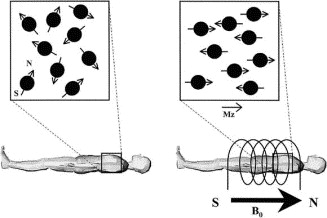
\includegraphics[width=0.5\linewidth]{imgs/B0 Magnetic Field.jpg}
     \caption{Protons align in parallel or antiparallel to the external field. Parallel alignment is a lower energy state, thus slightly more popular, leading to a net magnetisation vector (Mz). Figure from \cite{RobPio:99}}
\end{figure}
\subsection{RF Pulses}
The overall net magnetisation from all protons is represented by the vector \(\mathbf{M}=(M_x,M_y,M_z)\). At equilibrium, \(M_z\) is aligned with the static \(B_0\) field. The transverse components \(M_x\) and \(M_y\), which rotate about \(B_0\), are usually grouped into the complex notation \(M_{xy}=M_x+iM_y\).

The receiver coils measure transverse magnetisation \(M_{xy}\), not longitudinal magnetisation \(M_z\) directly. A perpendicular radio-frequency field \(B_1\), applied at the Larmor frequency, tips some or all of \(M_z\) into the transverse plane. This creates \(M_{xy}\), which precesses about \(B_0\) and induces a voltage in receiver coils placed perpendicular to the main field, as shown in Figure 2.2. The \(B_1\) pulses are called radio-frequency (RF) pulses because the Larmor frequency lies in the radio-frequency range. \cite{RobPio:99}\cite{MRI_Physics_Primer:12} 

The resulting angle between $M$ and $B_0$ is called the flip angle ($\alpha$) and can be calculated using:
\begin{equation}
    \alpha = \gamma \int B_1(t) \, dt
\end{equation}
\begin{figure}
    \centering
    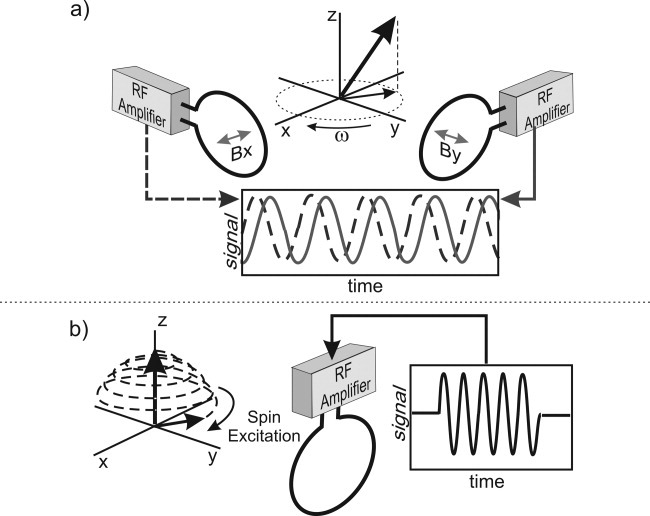
\includegraphics[width=0.5\linewidth]{imgs/mri_singal_generation.jpg}
    \caption{A voltage is induced via electromagnetic induction, making an MR signal. (A) The coils are perpendicular and can measure the phase and amplitude of the transverse magnetic vector. (B) RF pulses progressively "flip" the z-axis magnetisation vector into the transverse plane. 
    Figure from \cite{MRI_Physics_Primer:12}}
\end{figure}
\subsection{T1, T2 \& T2* Relaxation}
After an RF pulse is switched off, \(M_z\) recovers towards thermal
equilibrium along \(B_0\), while \(M_{xy}\) decays in the transverse plane
(the free induction decay). These are independent processes: longitudinal
relaxation transfers energy back to the surrounding lattice, while
transverse relaxation describes loss of phase coherence between spins.

Longitudinal, or spin-lattice, relaxation is characterised by \(T_1\): the
time taken for \(M_z\) to recover 63\% of the way back to its equilibrium
value \(M_0\) after excitation. Because this recovery depends on energy
exchange with the local molecular environment, \(T_1\) is an intrinsic
tissue parameter.\cite{RobPio:99}

Transverse, or spin-spin, relaxation describes the decay of \(M_{xy}\) as
spins lose phase coherence after excitation. Irreversible dephasing from
spin-spin interactions is characterised by \(T_2\), while reversible
dephasing from static \(B_0\) inhomogeneity is written as \(T_2'\). The
observed transverse decay \(T_2^*\) combines both effects:

\begin{equation}
    \frac{1}{T_2^*} = \frac{1}{T_2} + \frac{1}{T_2'}.
\end{equation}

A \(180^\circ\) refocusing pulse reverses the static dephasing term
\(T_2'\), which is why spin-echo sequences measure a signal governed
primarily by \(T_2\) relaxation. In biological tissue, \(T_2\) is generally
shorter than \(T_1\).\cite{MRI_Physics_Primer:12}

\begin{figure}
    \centering
    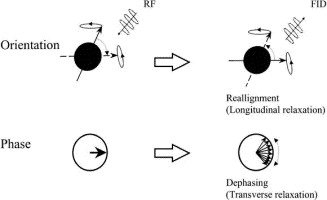
\includegraphics[width=0.5\linewidth]{imgs/relaxation_properties.jpg}
    \caption{\textbf{Upper Row:} Longitudinal relaxation (decreasing the flip angle). \\
    \textbf{Lower Row:} Transverse relaxation (spin dephasing) 
    Figure from \cite{RobPio:99}}
    \label{fig:relaxation-properties}
\end{figure}

\paragraph{Bloch-equation model.}
The Bloch equations formalise the relaxation behaviour above. In the
rotating frame at \(\omega_0\), with equilibrium magnetisation \(M_0\)
along \(+z\), the relaxation dynamics can be written as:

\begin{equation}
    \frac{dM_z}{dt} = -\frac{M_z - M_0}{T_1},
    \qquad
    \frac{dM_{xy}}{dt} =
    -\frac{M_{xy}}{T_2} + i\Delta\omega M_{xy}
\end{equation}

Here $\Delta\omega$ is the local off-resonance frequency relative to the
rotating frame. The first equation describes longitudinal recovery:
$M_z$ exponentially returns to $M_0$ with time constant $T_1$. The second
describes transverse decay: the magnitude of $M_{xy}$ falls with time
constant $T_2$, while off-resonance produces additional phase rotation.

Between RF pulses, these independent differential equations have the free-precession
solutions:

\begin{equation}
    M_z(t) = M_0 + \left(M_z(0) - M_0\right)e^{-t/T_1},
    \qquad
    \left|M_{xy}(t)\right| =
    \left|M_{xy}(0)\right|e^{-t/T_2}
\end{equation}

These are the signal-decay relationships used by the conventional quantitative 
MRI fitting methods used later in this work. Under the hard-pulse
approximation, an RF pulse is treated as an instantaneous rotation by flip
angle $\alpha$ about a transverse axis. If the longitudinal magnetisation
immediately before excitation is $M_z^-$, the pulse leaves
$\cos(\alpha)M_z^-$ on the longitudinal axis and tips
$\sin(\alpha)M_z^-$ into the transverse plane. The received signal is 
proportional to this transverse component.

After readout, the sequence models used in this work assume that residual
transverse magnetisation is removed by gradient spoiling or by relaxation
before the next acquisition block. The only state carried between shots is
therefore the scalar longitudinal magnetisation, updated by RF rotations and
$T_1$ recovery. This reduces the Bloch dynamics to simple recurrence
relations; without this assumption, transverse coherences would need to be
tracked explicitly using a coherence-pathway method such as Extended Phase
Graphs (EPG).

\subsection{Spatial Encoding \& K-Space}
Relaxation determines how much signal a spin can produce, but an image
also requires spatial localisation. MRI does not measure image pixels
directly. Instead, the scanner samples k-space: a spatial-frequency
representation of the image, shown in Figure~\ref{fig:kspace-representation}.
The centre sample of k-space, \(S(0,0)\), has no gradient moment along
either axis, so all spins contribute without a spatial phase ramp. It is
therefore the integral of the whole image, or mean signal,
conventionally called the DC term.

\begin{figure}
    \centering
    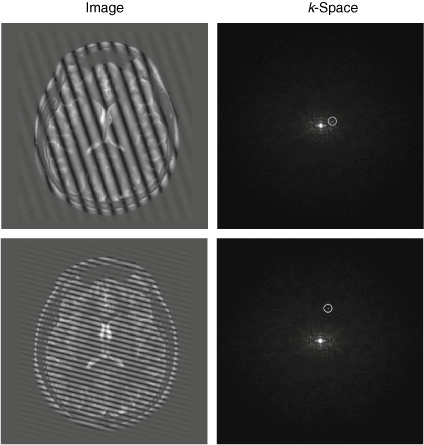
\includegraphics[width=0.55\linewidth]{imgs/kspace/k_space_indvidual_pixel_real.png}
    \caption{Image space and k-space are Fourier-pair representations of the same data: an MR image can be viewed either as a matrix of intensities \(I(x,y)\) or as spatial-frequency amplitudes \(S(k_x,k_y)\). Each k-space point weights a sinusoidal wave across the field of view; the vector angle \((k_x,k_y)\) sets the wave-pattern orientation, and its distance from the origin sets the spatial frequency. The centre of k-space contains low-spatial-frequency contrast and mean signal, while the outer samples contain high-spatial-frequency detail. Figure from \cite{buxton_fmri_2009}.}
    \label{fig:kspace-representation}
\end{figure}

Let \(G_x\), \(G_y\), and \(G_z\) denote magnetic-field gradients along
the scanner axes. These gradients make the Larmor frequency
position-dependent by varying the local field strength, providing the
spatial information missing from the raw MR signal.

The \(G_z\) gradient performs slice selection. During the RF pulse,
\(G_z\) maps \(z\)-position to Larmor frequency, so a narrow-band RF
pulse excites only the spins whose frequencies lie within the RF
bandwidth. This selects a thin slice of the object.

The in-plane coordinates are then encoded using \(G_y\) and \(G_x\). A
short \(G_y\) pulse before readout provides phase encoding: it gives
spins at different \(y\)-positions different accumulated phases. A
\(G_x\) gradient is kept on during ADC readout for frequency encoding:
successive samples trace spatial frequency along \(k_x\). Repeating the
sequence with different \(G_y\) amplitudes steps through \(k_y\), so each
repetition fills a different row of k-space.

% \begin{figure}
%     \centering
%     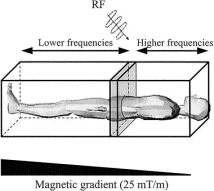
\includegraphics[width=0.5\linewidth]{imgs/slice_selection.jpg}
%     \caption{Slice selection using a narrow-band RF pulse applied during a gradient. Only spins whose shifted Larmor frequencies lie within the RF bandwidth are excited. Figure from \cite{RobPio:99}.}
%     \label{fig:slice-selection}
% \end{figure}

For a gradient waveform \(\mathbf{G}(t)\), the sampled k-space location
is determined by the accumulated gradient moment:

\begin{equation}
    \mathbf{k}(t) = \gamma\int_0^t \mathbf{G}(\tau)\,d\tau.
\end{equation}

Stronger or longer gradients move the acquisition further through
k-space. At a given k-space location, the acquired signal is

\begin{equation}
    S(\mathbf{k}) =
    \int m(\mathbf{r})e^{-i2\pi\mathbf{k}\cdot\mathbf{r}}\,d\mathbf{r}.
\end{equation}

Here \(m(\mathbf{r})\) is the transverse magnetisation at position
\(\mathbf{r}\). The exponential term applies a position-dependent phase
rotation to each complex \(M_{xy}\) contribution before the receiver sums
over the object. Changing \(\mathbf{k}\) changes this phase pattern, so
each measurement extracts a different spatial-frequency component of the
image. The image is recovered by applying an inverse Fourier transform to
the sampled k-space.

Two design quantities follow directly from this sampling geometry. The
k-space sample spacing determines the field of view:
\(\mathrm{FOV}=1/\Delta k\). If the object extends beyond this FOV, it
aliases back into the image. The k-space extent determines the nominal
pixel size, \(\Delta x=\mathrm{FOV}/N\approx 1/(2k_{\max})\). Acquiring
a wider k-space window improves spatial resolution, but it requires more
samples. In particular, higher \(k_y\) resolution means acquiring more
phase-encode rows, which usually requires additional sequence
repetitions.

\paragraph{FFT ordering.}
The Fourier relationship above defines the k-space/image-space mapping,
but not the array ordering used to store samples. KomaMRI returns
Cartesian ADC data in acquisition order, with the DC sample \(S(0,0)\)
near the centre of the stacked k-space matrix. For an even matrix size
\(N\), the standard acquisition convention samples one extra negative
line,
\[
    -N/2,\,-N/2+1,\,\dots,\,0,\,\dots,\,N/2-1,
\]
so for \(N=32\) this is \(-16,\dots,0,\dots,15\). DC therefore lies at
index \(N/2+1\) in one-based indexing. Standard FFT routines instead
expect DC at the first array index, so reconstruction requires

\[
    I = \mathrm{fftshift}\left(
        \mathrm{ifft}\left(\mathrm{ifftshift}(S)\right)
    \right),
\]

Here \(\mathrm{ifftshift}\) converts the centre-DC acquisition ordering
to FFT ordering, and \(\mathrm{fftshift}\) recentres the reconstructed
image. Without these shifts, the image is reconstructed under the wrong
indexing convention, causing a half-FOV shift and possible checkerboard
phase modulation.

\subsection{Gibbs (Truncation) Ringing}
\paragraph{Finite k-space support.}
The Fourier relationship is exact only if all of k-space is measured. In
practice, the acquisition covers a finite \(N_{pe}\times N_{fe}\)
rectangle. This is equivalent to multiplying the ideal infinite k-space
by a rectangular window. By the convolution theorem, multiplication in
k-space becomes convolution in image space:

\begin{equation}
    I_{\mathrm{recon}}(\mathbf{r})
    =
    I_{\mathrm{true}}(\mathbf{r}) * \mathrm{PSF}(\mathbf{r}).
\end{equation}

The point-spread function (PSF) is the Fourier transform of the sampling
window. For a one-dimensional rectangular window, it is the Dirichlet
kernel,

\begin{equation}
    \mathrm{PSF}(x) =
    \frac{\sin(\pi N x/\mathrm{FOV})}
         {N\sin(\pi x/\mathrm{FOV})}.
\end{equation}

This PSF has a narrow main lobe but slowly decaying side-lobes. At sharp
intensity transitions, such as the water--sphere boundaries in the
phantom, those side-lobes do not cancel and appear as Gibbs ringing.
Increasing \(N\) makes the ringing finer in physical units, but it does
not remove the side-lobes; the artefact is caused by the rectangular
truncation itself. The usual suppression method is apodisation, such as a
Hamming window, which down-weights outer k-space to reduce ringing at the
cost of a wider PSF and therefore slightly lower spatial resolution.
Appendix~\ref{app:kspace-apodisation} derives this trade-off, since it is
used directly by the phantom library's Hamming reconstruction option.


\subsection{Pulse Sequences}

A pulse sequence is the timed series of RF pulses, gradients, and signal
acquisitions that produces an image. Its timing parameters set the
image contrast and govern the trade-off between signal-to-noise ratio (SNR)
and scan time. The two most important are the repetition time (TR), the
interval between successive excitations, which controls $T_1$ weighting and
largely sets the total scan time, and the echo time (TE), the delay from
excitation to readout, which controls $T_2$ weighting. Choosing these values
is traditionally a manual craft: sequences are "handcrafted by MR experts, who
combined strong intuitions and an understanding of spin physics with
mathematical solutions of the Bloch equations"\cite{DLINMRI:24}. It is exactly
this hand-tuning of acquisition timings that the learned, adaptive approach of
this project seeks to automate.

\subsection{MRI Simulators}
Bloch-equation simulation is a mature area. KomaMRI, the Julia-based simulator
used in this project, is a high-performance, multi-threaded solver that sits
alongside the established JEMRIS~\cite{stoecker_jemris_2010} and
MRiLab~\cite{liu_mrilab_2017}, with the differentiable PyTorch framework
MRzero a further alternative~\cite{MRISeqSupLearning:21}. Its publication
benchmarked KomaMRI against both, reporting mean absolute signal differences
below 0.1\% versus JEMRIS with faster runtimes and better usability
scores~\cite{komaMRI:23}. Crucially, these are cross-simulator agreement checks
on short reference sequences, not validations of a quantitative pipeline. At
the long sequence times this project requires, KomaMRI produced systematically
inaccurate signals, biasing the fitted tissue parameters;
Chapter~\ref{ch:validating-komamri} diagnoses and fixes the cause.

\subsection{Magnetic Resonance Fingerprinting (MRF)}

Conventional MRI predominantly produces qualitative, ``weighted'' images where pixel intensity represents a relative contrast. This depends on acquisition parameters such as coil sensitivity, and makes it difficult to standardise across different scanners. In contrast, Quantitative MRI (qMRI) aims to measure the fundamental physical properties of tissues, such as the longitudinal ($T_1$) and transverse ($T_2$) relaxation times mentioned earlier. A significant advancement in this field is Magnetic Resonance Fingerprinting (MRF), which replaces traditional steady-state sequences with "pseudorandomized acquisition parameters". By varying the flip angles and repetition times ($T_R$) throughout the scan, MRF generates a unique signal evolution—or ``fingerprint''—for every tissue type. These signals are then pattern-matched against a pre-computed dictionary of Bloch equation simulations, allowing for the simultaneous and rapid mapping of multiple tissue properties in a single acquisition. For MR-guided radiotherapy, this quantitative approach offers the potential for ``biological gating'', where treatment adaptation is driven by functional changes in tumour physiology rather than just anatomical shifts. \cite{mehta_mrf_review:2019} \cite{Jordan_MRF_AUTO:21}

% Could use any of these as references
% [26] Ansorge R, Graves M. The physics and mathematics of MRI. Morgan & Claypool Publishers; 2016.
%[27] Haacke EM. Magnetic resonance imaging: physical principles and sequence design. (No Title). 1999.
% [28] Bernstein MA, King KF, Zhou XJ. Handbook of MRI pulse sequences. Elsevier; 2004.
% or this: MRI: CONNECTING THE DOTS https://iopscience.iop.org/book/mono/978-0-7503-1284-4

\section{Digital twins and phantoms for quantitative MRI}
\label{sec:bg-twins-phantoms}

Because the target of qMRI is a fitted physical parameter, an image can look
plausible while the fitted $T_1$ values are biased. Validating a qMRI method
therefore requires reference objects with known parameter values. Physical
phantoms fill this role: recent qMRI phantom reviews treat them as traceable
reference systems for repeatability studies, protocol comparison, and
cross-scanner validation, not merely as image-quality test
objects~\cite{keenan_phantoms_2024}. The most established example is the
ISMRM/NIST system phantom, designed as a common scanner-characterisation
baseline with SI-traceable reference materials spanning clinically relevant
$T_1$, $T_2$, and proton-density ranges, monitored long-term by a national
metrology institute~\cite{russek_system_phantom_characterization_2020}.
Chapter~\ref{ch:mri-system-phantom} builds a digital twin of exactly this
device.

Digital twins extend the reference idea from hardware to executable models. A
2026 systematic review of digital twinning in MRI defines a twin as a dynamic
virtual replica linked to its real-world counterpart through data,
simulation, and analytics, and maps 51 studies from
2020--2025~\cite{greggio_digital_twinning_mri_2026}. Two of its findings
locate this project. First, the MRI-twin literature concentrates on
diagnosis, treatment planning, and monitoring (63\% of studies); hardware,
protocol, and infrastructure applications --- the category this project
contributes to --- account for 20\% and are identified as underdeveloped.
Second, the review names barriers that this report confronts directly:
heterogeneity of MRI data across vendors, sequences, and field strengths; the
computational cost of physics simulation; and validation. This project
addresses them in a bounded setting --- a standardised phantom model, a
simulator validated by parameter recovery, and a multi-fidelity training loop
that attacks simulation cost. The term ``digital twin'' is used in a
correspondingly bounded sense throughout: the twin represents a calibration
phantom for simulation, validation, and policy training, not a patient or a
scanner connected to live clinical data.

Table~\ref{tab:bg-related-gaps} summarises how the approaches reviewed in
this chapter relate to the adaptive-qMRI problem and what each leaves
unresolved.

\begin{table}[!htbp]
\centering
\small
\setlength{\tabcolsep}{4pt}
\renewcommand{\arraystretch}{0.96}
\begin{tabularx}{\linewidth}{>{\raggedright\arraybackslash}p{3.4cm}
>{\raggedright\arraybackslash}X
>{\raggedright\arraybackslash}X}
\toprule
Related approach & Strength & Remaining gap for this project \\
\midrule
Physical qMRI phantoms~\cite{keenan_phantoms_2024,russek_system_phantom_characterization_2020} &
Known $T_1$/$T_2$/PD values; repeatable scanner and protocol validation &
A hardware object cannot generate randomised simulation episodes or cheap RL rollouts \\
\addlinespace
MRI digital twins~\cite{greggio_digital_twinning_mri_2026} &
Executable virtual replicas for prediction and optimisation &
Existing work targets diagnosis/treatment planning; protocol-level twins are underdeveloped \\
\addlinespace
MRI simulators~\cite{komaMRI:23,stoecker_jemris_2010,liu_mrilab_2017} &
Bloch-equation forward models; sequence testing before scanner execution &
Benchmarked on short reference sequences, not end-to-end qMRI recovery under long adaptive acquisitions \\
\addlinespace
Offline sequence optimisation~\cite{MRISeqSupLearning:21,Jordan_MRF_AUTO:21} &
Learns or optimises non-trivial acquisition schedules &
Schedule is fixed before the scan; no conditioning on the current fit \\
\addlinespace
Adaptive MR and RL scanner control~\cite{adaptive_mri:23,Walk_RL_CONTROL_MRI:19,zhu2018autoseq,pineda_active_mri_rl_2020} &
Closed-loop acquisition demonstrably helps &
Prior tasks differ: Bayesian T2/MRS adaptation, shape classification, 1-D physics, or k-space sampling --- not fitted $T_1$ mapping on a calibrated phantom \\
\bottomrule
\end{tabularx}
\caption{Related approaches, their strengths, and the gap each leaves for
closed-loop qMRI sequence design. The project combines the rows: an
executable phantom twin (Chapter~\ref{ch:mri-system-phantom}) drives a
validated simulator (Chapter~\ref{ch:validating-komamri}), and an RL agent is
trained and evaluated on the quantitative recovery objective
(Chapter~\ref{ch:adaptive-rl}).}
\label{tab:bg-related-gaps}
\end{table}

\section{Magnetic Resonance Linear Accelerator (MR-LINAC)}

The MR-LINAC couples real-time MR imaging with dose delivery, replacing the
pre-treatment 'snapshot' of conventional IGRT with a continuous feedback loop
that supports Adaptive Radiotherapy (ART). Imaging the patient on the table
lets clinicians correct for inter-fraction change and intra-fraction motion,
tightening the margins added around the target (in prostate cancer, planning
margins of ${\approx}2$\,mm) and so sparing healthy tissue\cite{ocanto_mr-linac:2024}.
Its clinical value is, however, throttled by two bottlenecks this project's
context touches: the extra acquisition time needed for high-quality imaging,
and the manual effort of on-table re-planning\cite{mrlinac_in_practice:23}.
AI-based auto-segmentation already addresses the contouring
load\cite{phillip_mri_seg:2020}, and the longer-term direction is to move
beyond anatomical contrast toward quantitative, biologically-targeted
acquisition --- the setting this project studies.

% mrilab - numberical mri simulator: https://leoliuf.github.io/MRiLab/
% paper: https://pmc.ncbi.nlm.nih.gov/articles/PMC5322984
% apparently komaMRI is easier to use
% not sure what Generalised Multi-Pool Exchange Tissue Model

\section{Deep Learning in MRI}
Long acquisition times represent a major barrier in clinical MRI, primarily due to the inherent trade-off between
image quality and speed of imaging. Indeed, the 3D images crucial for tumour delineation require longer acquisition times, which increases the risk of motion artifacts. There is a large body of research into reducing acquisition time while maintaining image quality. Notable breakthroughs include Parallel Imaging (multiple receiver coil arrays) and Compressed Sensing. Unfortunately, Parallel Imaging quickly reaches practical Signal-to-Noise Ratio (SNR) limits, while compressed sensing is prohibitively computationally expensive. \cite{DLINMRI:24}

To supplement, DL has been widely applied, both in research and through commercial products, to reduce imaging time and improve image quality. For example, DL is used in post-processing to remove noise, improve image resolution and reduce image inaccuracies (called artifacts) from patient movement or field inhomogenities (e.g. caused by metal patient implants or pacemakers). \cite{mri_questions:26}
\begin{figure}
\centering
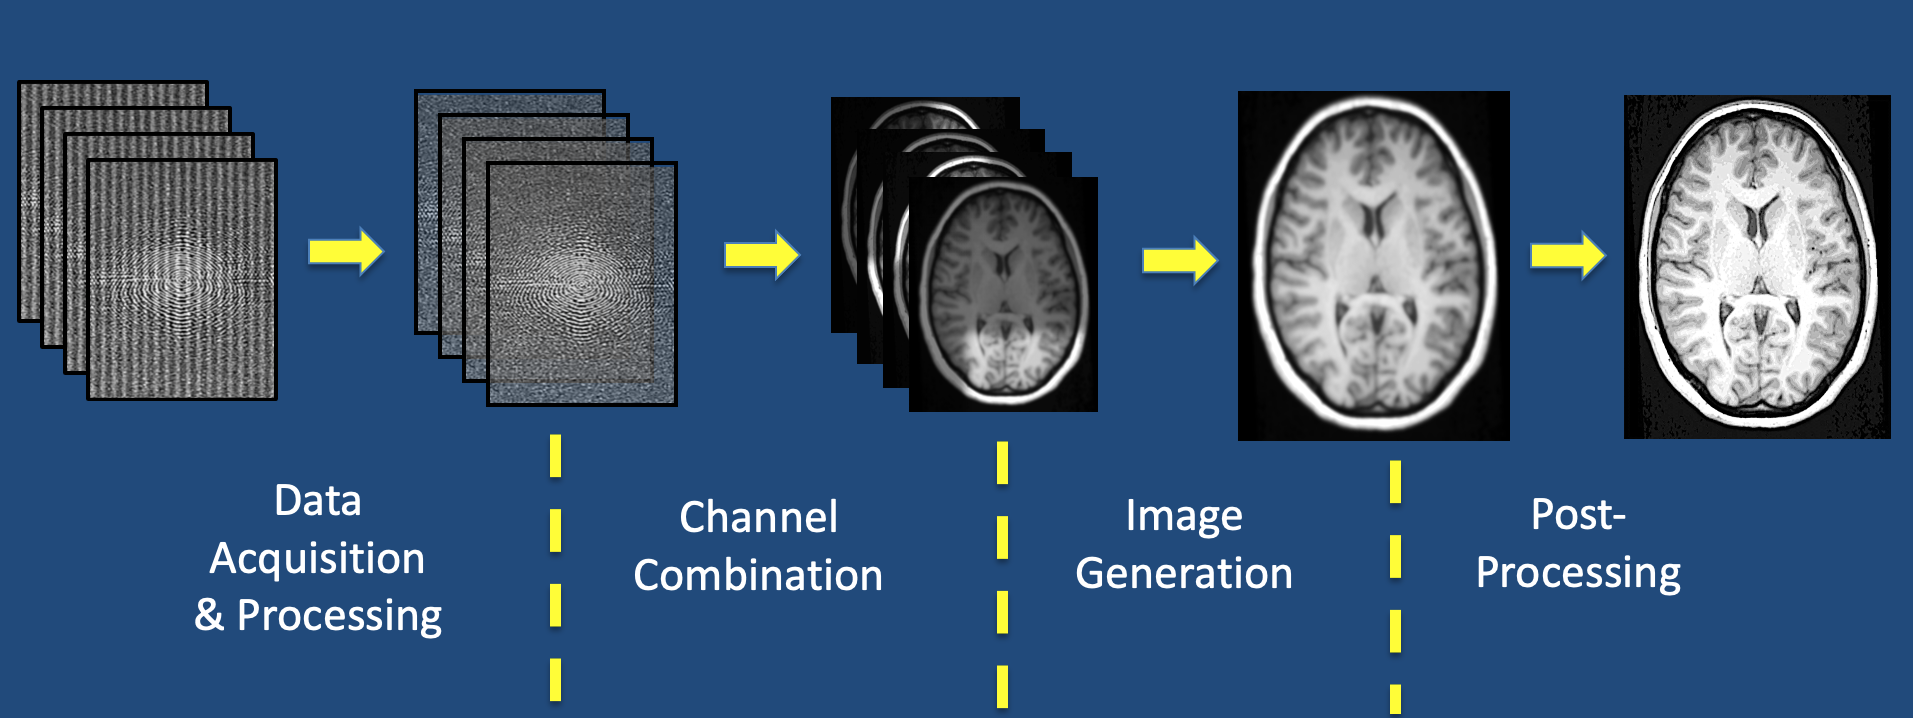
\includegraphics[width=0.8\columnwidth]{imgs/dl-spots-in-pipeline_orig.png}
\caption[MRI Image Pipeline]{Courtesy of Allen D. Elster, MRIquestions.com. \cite{mri_questions:26}}
\end{figure}
\subsection{Image Acquisition and Reconstruction using Deep Learning}
Post-processing operates only on the output image, which allows leveraging traditional imaging techniques (CNN, image kernels) as well as being vendor-neutral (so hardware-agnostic). However, not having the raw signal limits the information available.

This has given rise to more complex networks that replace both the Fast Fourier Transform algorithm used for reconstruction and post-processing to create higher quality images.

\subsection{Pulse sequence design}
Recent research has explored the use of artificial intelligence to optimise the underlying physics of MR acquisition through the autonomous design of pulse sequences. Two differing approaches have been tested: an RL game-based approach and a more traditional supervised learning approach.

The MRzero framework introduces a supervised learning approach that treats the entire scanning and reconstruction pipeline as a fully differentiable system. By simulating RF events, gradient moments, and delay times through a Bloch equation layer, the model can be optimised directly against a target contrast of interest (e.g. a $T_1$ contrast map). The cost function that was optimised by the model took into account: data fidelity, Specific Absorption Rate (SAR) penalties and scan time. The researchers successfully demonstrated that MRzero could "learn" to replicate conventional gradient-echo sequences from scratch. This was then successfully tested on a clinical 3T scanner for in vivo human brain imaging. This demonstrates that deep learning-derived sequences are clinically viable and can be optimised for specific hardware constraints.\cite{MRISeqSupLearning:21}

By recasting pulse sequence development as a ``game of perfect information,'' researchers have implemented a reinforcement learning (RL) framework where an AI agent interacts with a Bloch equation-based physics simulator to generate novel sequence actions. This approach utilises a Bayesian derivative of RL, employing Gaussian processes and Bayesian neural networks to navigate the non-linear dynamics of nuclear magnetisation and maximise an acquisition function based on image reconstruction accuracy. Preliminary 1-D experiments demonstrate that such agents can independently ``discover'' canonical sequences, such as the gradient echo, and generate novel pulse sequences that approximate Fourier spatial encoding. While this was a 1-D experiment, further exploration could yield novel pulse sequences that reduce acquisition time and maximise SNR, alleviating the current acquisition bottleneck faced by the MR-Linac.\cite{zhu2018autoseq}


%The optimisation of Magnetic Resonance Fingerprinting (MRF) represents a highly non-convex problem, often involving thousands of tunable parameters across flip angles and repetition times ($T_R$). Jordan et al. \cite{Jordan_MRF_AUTO:21} developed an automated design framework that moves beyond simple statistical noise models by incorporating an accelerated "digital phantom" that explicitly simulates systematic errors from Fourier undersampling and phase variation. By utilising substochastic Monte Carlo and simulated annealing algorithms, the researchers discovered non-intuitive pulse sequences—characterised by "spiked" $T_R$ durations—that achieved a fourfold reduction in scan time compared to expert-designed sequences while maintaining equivalent precision in $T_1$ and $T_2$ estimation. Crucially, these algorithmically discovered sequences demonstrated intrinsic robustness against shading artifacts caused by $B_0$ and $B_1$ field inhomogeneities. This suggests that automated physics-inspired design can produce protocols that are not only faster but also more resilient to the hardware-induced distortions common in hybrid systems like the MR-LINAC.

\begin{figure}
    \centering
    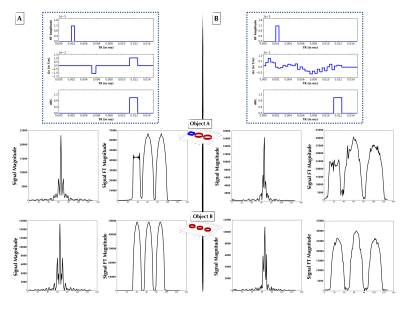
\includegraphics[width=0.5\linewidth]{imgs/AUTOSEQ_RES.png}
    \caption{(B) Novel pulse sequence successfully developed by AUTOSEQ to mimic a gradient echo sequence. Figure from \cite{zhu2018autoseq}}
    \label{fig:autoseq-gradient-echo}
\end{figure}

\subsection{Adaptive MRI acquisition}
The above work focuses on the design of novel, but ultimately static pulse sequences. Instead, Adaptive MR is a promising new research direction. Here, a probability distribution of the tissue parameter of interest (e.g. $T_2$) is continuously updated with each new reading. The next pulse sequence is chosen based on the estimate of $T_2$. This has been shown to accelerate acquisition time by a factor of 2.5. This is a general paradigm shift in pulse sequence design that motivates and validates further exploration of adaptive MR.\cite{adaptive_mri:23}

Adaptive MR also has the potential to be combined with RL to autonomously control in real-time MRI hardware. Walker-Samuel demonstrated this by using a Deep Deterministic Policy Gradient (DDPG) algorithm to control an MRI simulation environment where the acquisition process had been turned into a reward-based game. The RL agent was tasked with identifying phantom shapes while being penalised for increased acquisition time. This forces the system to optimise the trade-off between Signal-to-Noise Ratio (SNR) and image acquisition time. Notably, the agent autonomously learned to perform "active sensing," acquiring only four to six outer lines of $k$-space and dynamically adjusting $T_E$, $T_R$, and flip angles to act as an edge detector. With a reported shape-classification accuracy of 99.8\%, this research suggests that RL-controlled scanners could move beyond human-readable imaging to perform high-speed, task-specific "autonomous sensing". However, this was purely simulation-based and a very simple task, whether this method can be applied to more complex situations is unproven.

A separate active-acquisition literature applies RL to k-space sampling:
Pineda et al.\ train a policy that selects which k-space lines to acquire
next so that an undersampled reconstruction improves
fastest~\cite{pineda_active_mri_rl_2020}. This work also treats MRI
acquisition as a sequential decision problem, but it controls a different
object: sampling locations under a reconstruction-quality objective. It does
not choose relaxation-preparation timings such as TI and TR, and it does not
optimise fitted quantitative parameter accuracy --- the control problem and
objective of this project.

\subsection{Reinforcement Learning and PPO for Adaptive Acquisition}
Reinforcement learning (RL) studies problems where an agent improves its
behaviour by interacting with an environment. At each step the agent observes
the current state of the environment, chooses an action, and receives a scalar
reward. The objective is not to predict a labelled target directly, as in
supervised learning, but to learn a policy that selects actions leading to high
cumulative reward.\cite{sutton_barto_rl_2018}

The standard mathematical model is a Markov decision process (MDP),

\begin{equation}
\mathcal{M} = (\mathcal{S}, \mathcal{A}, P, R, \rho_0, \gamma),
\end{equation}

where $\mathcal{S}$ is the state space, $\mathcal{A}$ is the action space,
$P(s_{t+1}\mid s_t,a_t)$ is the transition model, $R$ is the reward function,
$\rho_0$ is the initial-state distribution, and $\gamma \in [0,1]$ is the
discount factor. A trajectory is a sequence

\begin{equation}
\tau = (s_0, a_0, r_0, s_1, a_1, r_1, \ldots).
\end{equation}

In this project, the environment is the simulated adaptive qMRI acquisition
loop. A state contains the information available to the agent so far, such as
the current acquisition history and the current estimate of the phantom
parameters. An action specifies the next acquisition choice, for example timing
and RF parameters such as inversion time, echo time, repetition time, and flip
angle. The simulator then returns reconstructed measurements and a reward based
on whether the new acquisition improves the quantitative parameter estimate,
typically measured through reduction in $T_1$ error.

For a stochastic policy $\pi_\theta(a\mid s)$ with parameters $\theta$, the
return from time $t$ is

\begin{equation}
G_t = \sum_{k=0}^{T-t} \gamma^k r_{t+k}.
\end{equation}

The RL objective is to choose policy parameters that maximise expected return:

\begin{equation}
J(\theta) = \mathbb{E}_{\tau \sim \pi_\theta}[G_0].
\end{equation}

The expectation is over trajectories generated by the current policy interacting
with the environment. This is important in simulation-in-the-loop MRI: the
training data are not a fixed dataset. They are samples produced by repeatedly
running the current policy, simulating the resulting sequence, reconstructing
the image, fitting the tissue parameters, and computing the reward.

\subsubsection{Proximal policy optimisation}
This project optimises the policy with Proximal Policy Optimisation
(PPO)~\cite{schulman_ppo_2017}, an on-policy policy-gradient method. Policy
gradients estimate $\nabla_\theta J(\theta)$ from sampled rollouts, weighting
each sampled action by an advantage estimate $\hat{A}_t$ that measures whether
it beat the return the policy already expected; the advantages are computed by
Generalised Advantage Estimation~\cite{schulman_gae_2016} from a learned critic
$V_\phi(s)$. Crucially, this gradient flows only through the differentiable
policy $\log\pi_\theta(a_t\mid s_t)$ and not through the environment, so KomaMRI
can stay a black-box physics simulator used only to sample transitions and
rewards. A plain policy-gradient step can move the policy too far and
invalidate the on-policy batch; PPO prevents this with a clipped surrogate
objective,

\begin{equation}
L^{\mathrm{CLIP}}(\theta)
=
\mathbb{E}_t
\left[
\min
\left(
    r_t(\theta)\hat{A}_t,
    \operatorname{clip}
    \left(r_t(\theta), 1-\epsilon, 1+\epsilon\right)
    \hat{A}_t
\right)
\right],
\qquad
r_t(\theta) =
\frac{\pi_\theta(a_t\mid s_t)}
     {\pi_{\theta_{\mathrm{old}}}(a_t\mid s_t)},
\end{equation}

where the ratio $r_t(\theta)$ compares the new and old action probabilities and
$\epsilon$ bounds how far one update may move them. The full objective adds a
critic loss and an entropy bonus. The policy-gradient derivation, the
value/advantage definitions, GAE, and the complete objective are given in
Appendix~\ref{app:rl-background}.

PPO suits adaptive qMRI for three reasons: it handles continuous action spaces
(the sequence timings), it explores stochastically while the clipped objective
prevents sudden policy collapse, and its on-policy simplicity makes the
physics-and-reward path easier to debug than an off-policy learner. The cost is
sample efficiency: every update needs fresh rollouts, and one rollout step here
is not a cheap game transition but a full MR sequence build, KomaMRI Bloch
simulation, image reconstruction, ROI extraction, $T_1$ fit, and reward
evaluation. The number of simulator calls is therefore the dominant training
bottleneck, which is what motivates the multi-fidelity training loop of
Chapter~\ref{ch:adaptive-rl}.

\subsubsection{Recurrent policies for partial observability}
The PPO actor and critic above are feed-forward networks that map the current
observation $s_t$ to an action distribution and a value. This implicitly
assumes $s_t$ is a sufficient statistic of the history, i.e.\ the Markov
property holds. When the observation does not capture everything relevant about
the past, the problem is a partially observed MDP (POMDP) and a memoryless
policy can be suboptimal. Adaptive qMRI is partially observed in exactly this
way: a compact observation of the current fitted estimates and remaining budget
does not record which acquisition timings have already been played, yet two
histories with the same current fit can carry different information for the next
block.

A recurrent policy adds an internal memory. The feed-forward trunk is preceded
by a recurrent network, here a Long Short-Term Memory (LSTM)
cell~\cite{hochreiter_lstm_1997}, that maintains a hidden state $h_t$ updated
each step from the previous state and the current observation,
$h_t = \mathrm{LSTM}(h_{t-1}, s_t)$. The action and value are conditioned on
$h_t$ rather than $s_t$ alone, so the policy can summarise the acquisition
history into $h_t$ and condition the next timing on it; the LSTM's gating lets
it retain information over many steps without the vanishing gradients of a
plain recurrent network. Training uses the recurrent variant of PPO, identical
to the above except that rollouts store hidden states and gradients are
propagated back through each rollout's recurrent steps (truncated
backpropagation through time). Chapter~\ref{ch:adaptive-rl} evaluates such a
policy as an ablation against the compact feed-forward observation, testing
whether explicit memory of the acquisition history improves adaptive timing.

\section{Summary}
\label{sec:bg-summary}

The MRI physics above (relaxation, spatial encoding, pulse sequences)
underpins the simulator and fitter of
Chapters~\ref{ch:mri-system-phantom}--\ref{ch:validating-komamri}, while the
deep-learning and reinforcement-learning sections position the adaptive
contribution of Chapter~\ref{ch:adaptive-rl}. The related work also exposes
the gaps this project targets, summarised in
Table~\ref{tab:bg-related-gaps}. Existing adaptive-MRI and automated
sequence-design work is either \emph{offline} --- the schedule is fixed
before the scan, as in magnetic resonance fingerprinting and
MRzero~\cite{MRISeqSupLearning:21} --- or, where it is closed-loop, is
validated on tasks other than calibrated quantitative mapping, such as
AUTOSEQ's 1-D physics simulation~\cite{zhu2018autoseq}, Walker-Samuel's
shape classification~\cite{Walk_RL_CONTROL_MRI:19}, or k-space sampling for
reconstruction quality~\cite{pineda_active_mri_rl_2020}. On the
infrastructure side, qMRI phantoms provide traceable ground truth but no
training episodes~\cite{keenan_phantoms_2024}, MRI digital twins remain
concentrated on diagnosis rather than protocol
development~\cite{greggio_digital_twinning_mri_2026}, and simulator
benchmarks stop short of end-to-end quantitative recovery
tests~\cite{komaMRI:23}. No prior work pairs an observation-conditioned RL
policy with a validated digital-twin simulator and a fitted-$T_1$ objective,
nor confronts the simulation-cost wall a Bloch solver in the training loop
creates; these two gaps motivate C1--C3 and the achievements that follow.

%"The pulse sequence design task was traditionally handcrafted by MR experts, who combined strong intuitions and an understanding of spin physics with mathematical solutions of the Bloch equations. While a remarkable number of contrast mechanisms and imaging schedules have been developed since the invention of MRI, the reliance on solvable differential equations severely limits our ability to reach a globally optimised schedule and reduce the scan time."\cite{DLINMRI:24}

% MRI QUESTIONS
%By comparison to post-processing methods, reconstruction-based AI has greater potential because it can utilise raw k-space data as well as other information such as coil sensitivities and phase. AI methods may even interact dynamically with the process of image acquisition.  For example, AI may be used to stop image acquisition once a certain threshold has been reached or to recognise corrupted data samples and repeat them.  
%Although generic techniques have been developed, for the most part AI-based reconstruction methods are vendor-dependent and highly proprietary. Examples include Siemens' Deep Resolve, GE's Air™Recon DL, and Philips' SmartSpeed.  Based on sales literature and discussions with industry insiders, these vendor-based techniques are all most useful in undersampled parallel imaging applications. Deep learning methodology may begin at the level of signals from individual coils before they are combined using information about individual coil sensitivities and noise maps. DL may also be applied to fully combined complex data during the k-space reconstruction process. The desired signal-to-noise level from this DL-enhanced hybrid construction can be adjusted by a radiologist-selectable tuning parameter (low/medium/high).
